
\documentclass[a4paper, 12pt]{article}
\usepackage[utf8]{inputenc}
\usepackage[T1]{fontenc}
\usepackage{lmodern}
\usepackage[french]{babel}
\usepackage{amsmath, amssymb, amsthm, mathtools, mathrsfs}
\usepackage[top=1.5cm, bottom=1.5cm, left=1.5cm, right=1.5cm]{geometry}
\usepackage[colorlinks=true]{hyperref} 
\hypersetup{urlcolor=blue, citecolor=red} 
\usepackage[all]{xy} 
\usepackage{graphicx} 
\usepackage{enumitem}
\usepackage{authblk}
\usepackage[export]{adjustbox}
\usepackage{float}
\usepackage[most]{tcolorbox}
\usepackage{chngcntr}

\counterwithin{figure}{section}

\newtcolorbox{mybox}{colback=black!5!white,colframe=black,
  boxrule=0.8mm,arc=4mm,boxsep=5pt}



\title{
    \Large Rapport Mini-Projet – Partie \uppercase\expandafter{\romannumeral 2}\\
    \textbf{La Maison de la Culture}
} 

\author{
    WENDELS Jérémy \\
    THIEFFRY Raphaël
}
\affil{Université Paris-Saclay - UFR des Sciences}


\newcommand{\figZoom}[1]{
\begin{figure}[H]
    \raggedleft
    \includegraphics[width=5cm]{./images/#1.png}
\end{figure}
} 
\newcommand{\fig}[2]{
\figZoom{BDD_#1}
\begin{figure}[H]
    \centering
    \includegraphics[width=\textwidth, max height=9cm]{./images/#1.png}
    \protect\caption{#2} 
\end{figure}
}


\date{\today}

\begin{document}

    \maketitle
    \tableofcontents

    \newpage

    \section{Résultat}
    \begin{mybox}
        \begin{figure}[H]
            \centering
            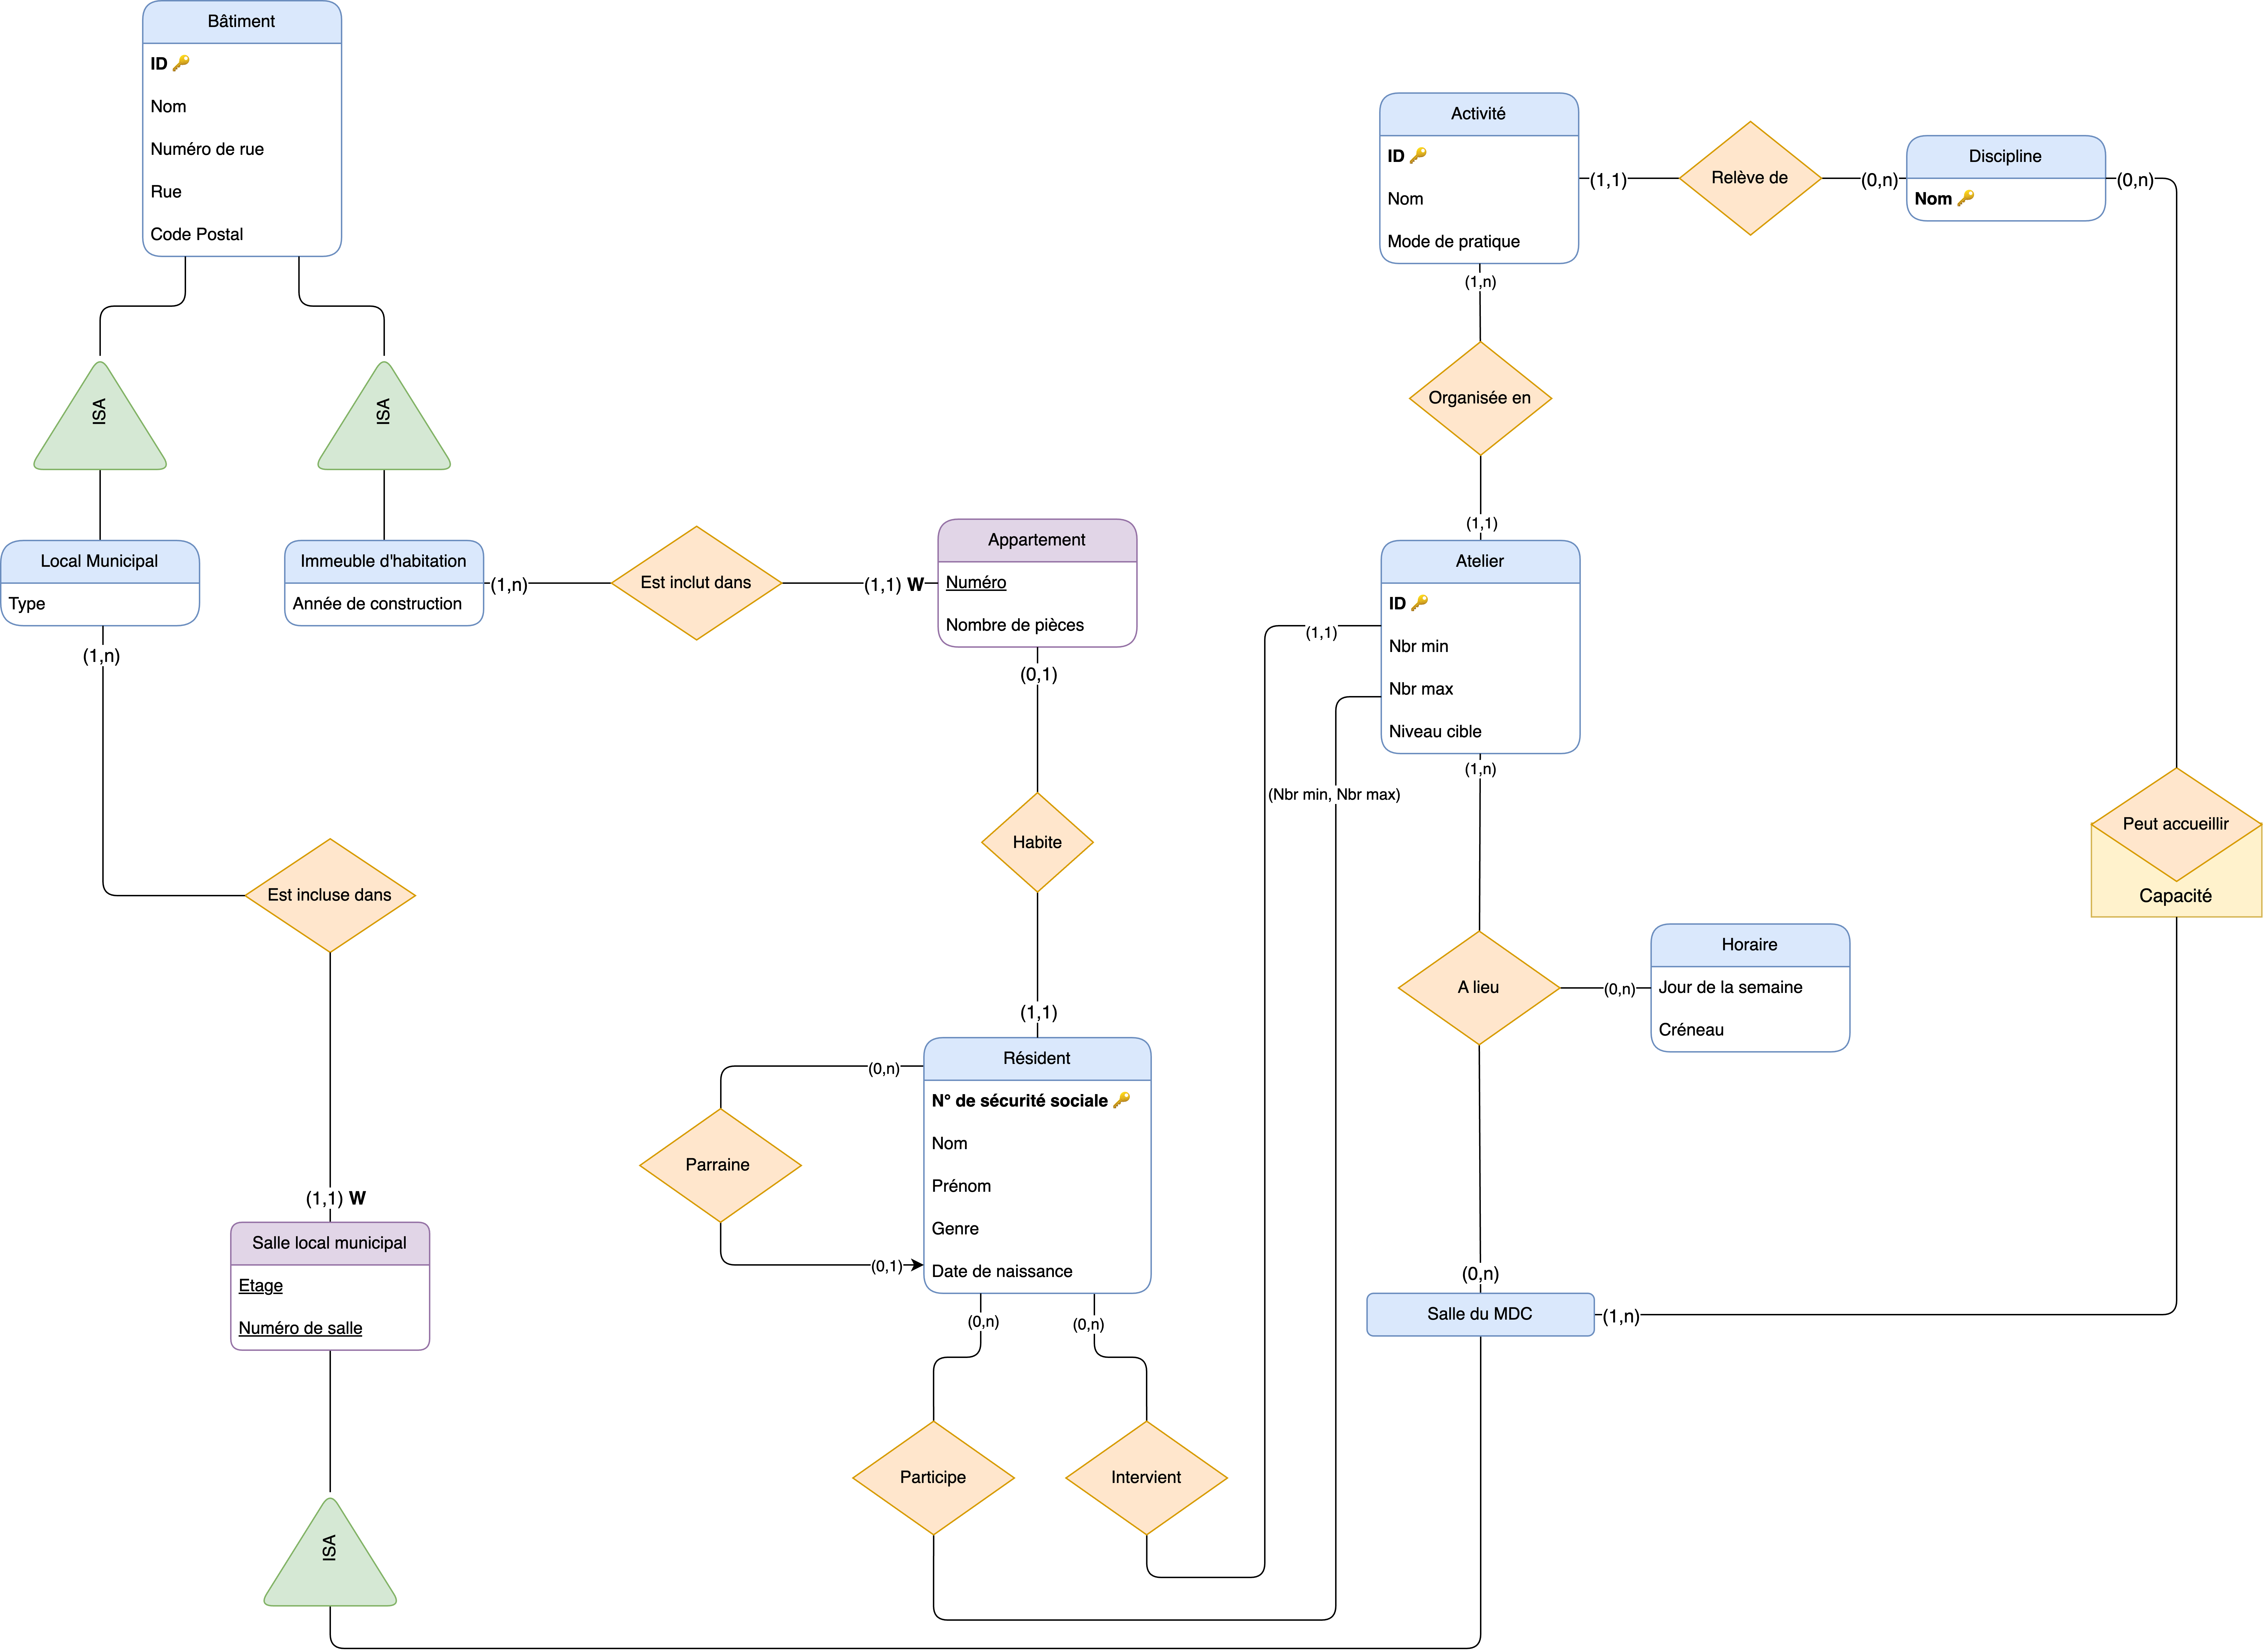
\includegraphics[width=\textwidth]{./images/BDD.png}
            \protect\caption{Schéma E/A final}
        \end{figure}
    \end{mybox}
    % lien vers l'image
    % pas de tabulation
    
    \noindent\href{https://www.jwendels.fr/BDD.svg}{Ouvrir/Télécharger l'image en SVG}
    \\
    \href{https://www.jwendels.fr/BDD.png}{Ouvrir/Télécharger l'image en PNG}

    \newpage

    \section{Explications}

        \subsection{Association Activité et Discipline}
        \begin{mybox}
            
            \fig{fig1}{Activité et Discipline}
            Comme on peut le voir, nous avons créé une entité Activité qui est liée à une (et une seule) entité Discipline, d'où la cardinalité $(1,1)$. Une discipline peut être liée à plusieurs activités (ou aucune). Nous avons donc une cardinalité $(0,n)$.
            
            Notons qu'ici, discipline est une entité à part (ie : n'est pas un attribut d'activité) pour des raisons que nous preciserons plus tard.
        \end{mybox}
        \newpage
        \subsection{Association Activité et Atelier}
        \begin{mybox}
            \fig{fig2}{Activité et Atelier}

            Là aussi, nous avons relié activité à un atelier. Pour une activité, il peut y avoir plusieurs ateliers (comme mentionné dans le sujet) (ie cardinalité $(1, n)$). Nous avons supposé que pour un atelier donné, il y avait forcement au moins un atelier sinon l'activité n'a pas de sens.

            Réciproquement, un atelier relève forcément d'une et une seule activité, comme mentionné dans le sujet (ie cardinalité $(1, 1)$).

            Les attributs sont tels qu'énoncés dans le sujet.
        \end{mybox}
        \newpage
        \subsection{Association Atelier, Horaire et Salle du MdC}
        \begin{mybox}
            \fig{fig3}{Atelier, Horaire et Salle du MdC}
            Ici, nous avons une "triple association" reliant une entité appelée `horaire`, à notre entité `atelier`, et à une salle.
            
            Cette association représente en quelques sortes les réservations. 
            
            On comprend ainsi qu'un atelier dispose nécessairement d'au moins une réservation (= horaire+salle), qu'il peut très bien exister des horaires sans salles réservées pour des ateliers. Aussi, une salle peut très bien n'être associé à aucun atelier pour un horaire donné.
            Ceci explique donc les cardinalités.
            
            D'autre part, notons que sur le sujet, il est indiqué qu'un atelier peut avoir lieu plusieurs jours par semaine mais pas deux fois le même jour. Aussi, deux ateliers ne peuvent pas avoir lieu dans la même salle au même horaire. Ce sont des contraintes qu'il faudra gérer quand nous nous occuperons des schémas relationnels.

            Enfin, détail important, ici `salle du MdC` n'a pas d'attribut car il hérite d'une autre entité que nous verrons plus tard.
        \end{mybox}
            

        \subsection{Association Discipline et Salle du MdC}
        \begin{mybox}
            \fig{fig4}{Discipline et Salle du MdC}
        On voit aussi que salle MdC est relié à l'entité discipline avec l'attribut d'association `capacité`' qui dépend de la discipline justement.
        C'est la raison pour laquelle discipline est une entité à part    
        
        \end{mybox}


        \subsection{Entité Bâtiment}
        \begin{mybox}
            \fig{fig5}{Bâtiment et ses ISA} 
            Pour la structure d'un batiment, nous avons réuni les attributs communs aux bâtiments publics et aux bâtiments d'habitation.
            L'adresse étant unique et ayant un format plutôt simple, nous avons jugé que la présenter sous forme d'attributs était pertinent et simplifiait le schéma.

            Les bâtiments publics (resp. d'habitation) héritent de cette entité bâtiment pour simplifier leurs attributs. On a donc un local municipal avec un attribut type, et un local d'habitation avec un attribut année de construction.

        \end{mybox}
        
        \subsection{Entité Salle local municipal}
        \begin{mybox}
            \fig{fig6}{Salle local municipal}
            Dans cette partie, ce qui saute aux yeux c'est que nous avons fait le choix de faire de la salle une entité faible du local. En effet, les clefs faibles de `salle local municipal` ne permettent que de décrire la salle dans l'enceinte d'un bâtiment donné. C'est pourquoi pour identifier une salle municipale de manière unique, il faut y adjoindre la clef du bâtiment (ID).
            Un local comporte au moins une salle sinon c'est absurde.

            Enfin, nous avons fait le choix d'avoir une entité `Salle local municipal` qui soit distincte de `Salle du MdC`. En effet, on peut très bien imaginer que la mairie dispose de salles qui ne sont pas dédiée au MdC.

            Pour conclure cette partie, on devine donc aisément que `Salle du MdC` hérite de `Salle de local municipal` au sens où elle a les mêmes attributs, mais a des associations différentes de `Salle de local municipal`

            La contrainte sur l'étage et le n° de salle donné dans le sujet est respectée car si on avait deux salles distinctes avec le même numéro au même étage, cela ne formerait plus une clef faible de `Salle local municipal`.
            \begin{figure}[H]
                \centering
                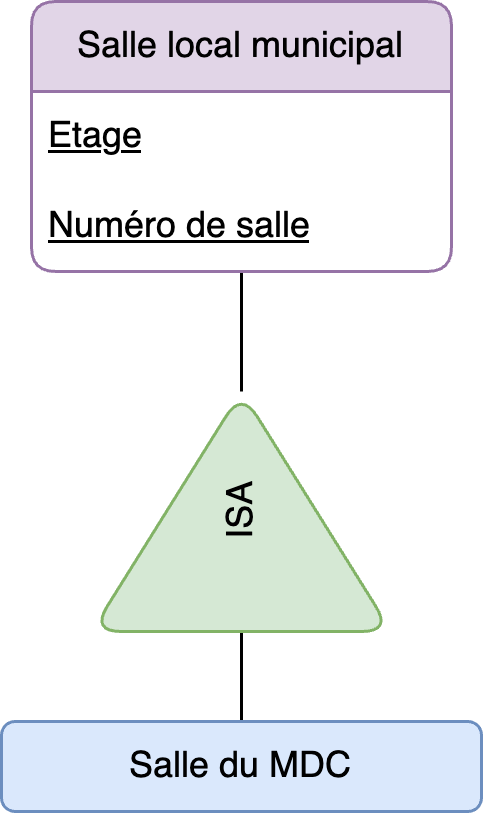
\includegraphics[width=\textwidth, max height=6cm]{./images/fig6_1.png}
                \caption{Salle du MdC hérite de Salle de local municipal}
            \end{figure}

        \end{mybox}

        \subsection{Association Immeuble d'habitation et Appartement}
        \begin{mybox}
            \fig{fig7}{Immeuble d'habitation et Appartement}
            De manière similaire, appartement est évidemment une entité faible de immeuble d'habitation. Le numéro d'appartement est la clef faible de l'appartement dans la mesure où elle permet d'identifier celui ci à l'intérieur d'un bâtiment donné
            Un immeuble a forcément au moins un appartement, et un appartement est inclus strictement dans un et un seul bâtiment (ie cardinalité $(1,1)$)
        \end{mybox}

        \subsection{Association Résident et Appartement}
        \begin{mybox}
            \fig{fig8}{Résident et Appartement}
            Un résident vit nécessairement dans un appartement, mais la réciproque n'est pas valable : un appartement en vente n'est pas forcément habité. D'où les cardinalités visibles sur le schéma. Chaque n°de sécu identifié chaque résident de manière unique, ça forme donc une clef de l'entité résident.
            
            Par ailleurs, cette relation nous fournit l'information concernant l'adresse du résident. En effet, l'adresse est une information contenue dans les attributs de `bâtiment` et de `appartemment` (un appartement est identifiable par l'ID du bâtiment et le numero d'appartement).
        \end{mybox}
        
        
        \subsection{Association Résident et Atelier + Parainage}
        \begin{mybox}
            \fig{fig9}{Résident et Atelier + Parainage}
            Maintenant autour de résident, voyons qu'il existe plusieurs associations. Commençons par parrainer, la seule association réfléxive. Un résident peut parrainer de 0 à n individus pour adhérer à la MdC. Réciproquement, un résident peut se faire parrainer 1 fois au plus par un autre résident.

            Ensuite, résident est relié à atelier. En effet, il peut être participant ou intervenant d'un atelier. Les contraintes concernant ces associations, à savoir qu'on ne peut pas être participant et intervenant dans le même atelier, ne peuvent pas être décrites dans le schéma c'est pourquoi il faudra s'en charger au moment du schéma relationnel.

            Puisque qu'un atelier dispose d'un intervenant strictement, cela explique la cardinalité $(1,1)$ du côté de `atelier`. De même, un atelier a un nombre de participants borné entre min et max, d'où la cardinalité visible sur le schéma.
            Un résident peut participer/intervenir à autant d'ateliers qu'il veut, dont 0. D'où les cardinalités $(0,n)$ coté résident. 
        \end{mybox}

\end{document}


% plusieurs choses possible : Une partie `EN BREF`, et échanger sens de certaines associations pour la lisibilité
